\chapter{関連研究}
\label{CRelatedWork}

%本研究で対象としている複眼の偽瞳孔現象をコンピュータグラフィックスの分野で扱った研究は未だ存在しない。
本研究では、複眼の偽瞳孔現象を対象としている。
偽瞳孔は複眼表面の微細構造によって巨視的に現れる模様であり、偽瞳孔をコンピュータグラフィックスの分野で扱った研究は未だ存在しない。
しかしながら、複眼同様に表面の微細構造を有している材質などのレンダリングを扱った研究は少なからず存在するため、それらを紹介する。

\section{微細構造を扱った研究}
\label{SMicrostructure}

表面微細構造をもつ物質をレンダリングする研究が過去にいくつか行われている。

\subsection{マイクロファセットモデル}

表面のマイクロファセット(microfacet)構造の例として車の塗装のようにざらついたようなきらめきを持つ材質がある。
こうした材質をレンダリングする手法として、G\"{u}ntherら\cite{}はノーマルマップ(normal map: 法線マップ)を利用し、Rumpら\cite{rump-2008-photo-realistic}は測定したテクスチャを用いた手法をそれぞれ提唱している。

%% \begin{figure}[htbp]
%%   \centering
%%   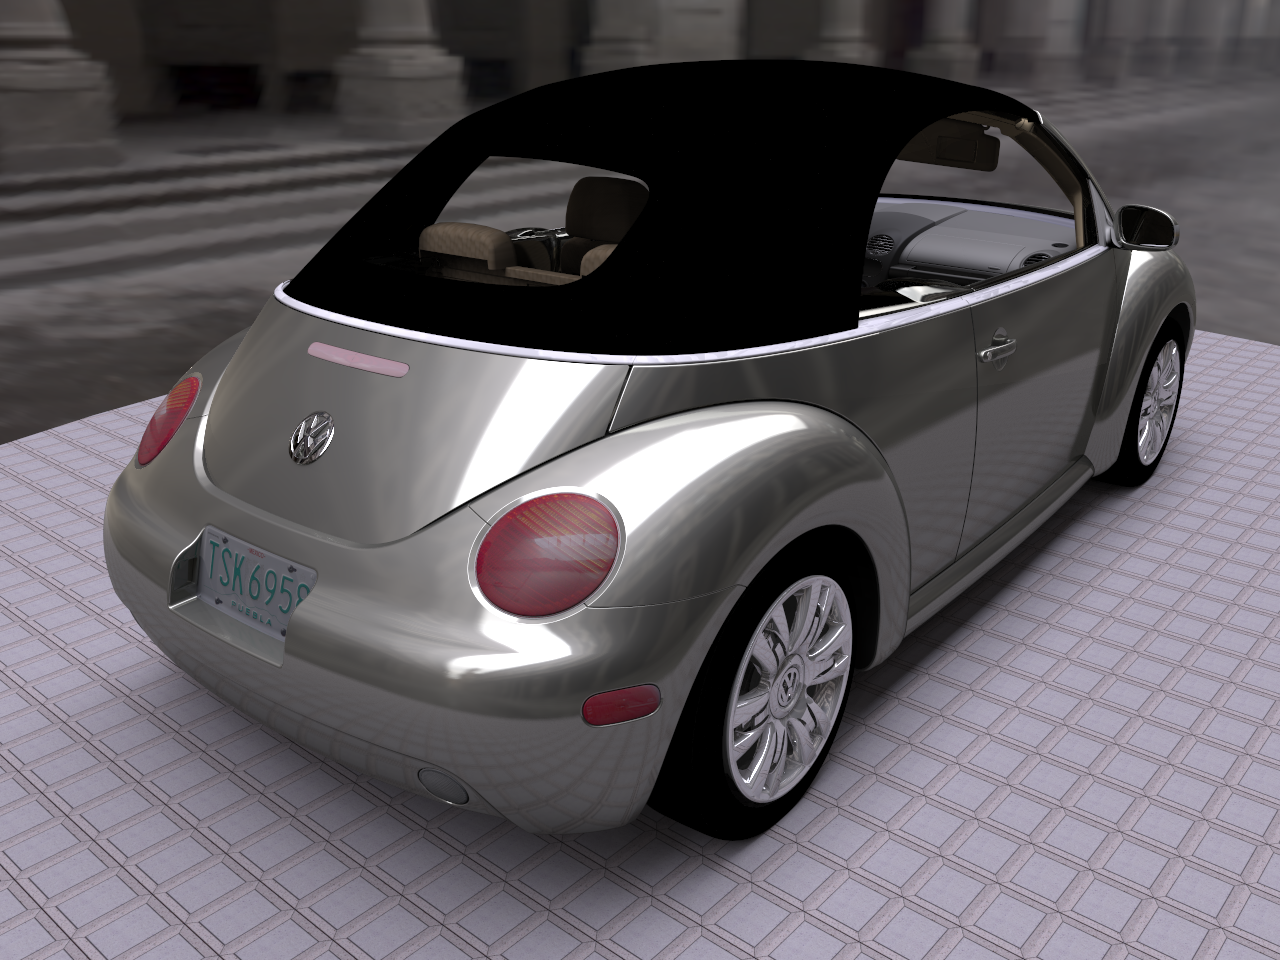
\includegraphics[width=3.5in]{./img/back_hq.png}
%%   \caption{guntherのやつ}
%%   \label{F}
%% \end{figure}

\begin{figure}[htbp]
 \begin{minipage}{0.4\hsize}
  \begin{center}
   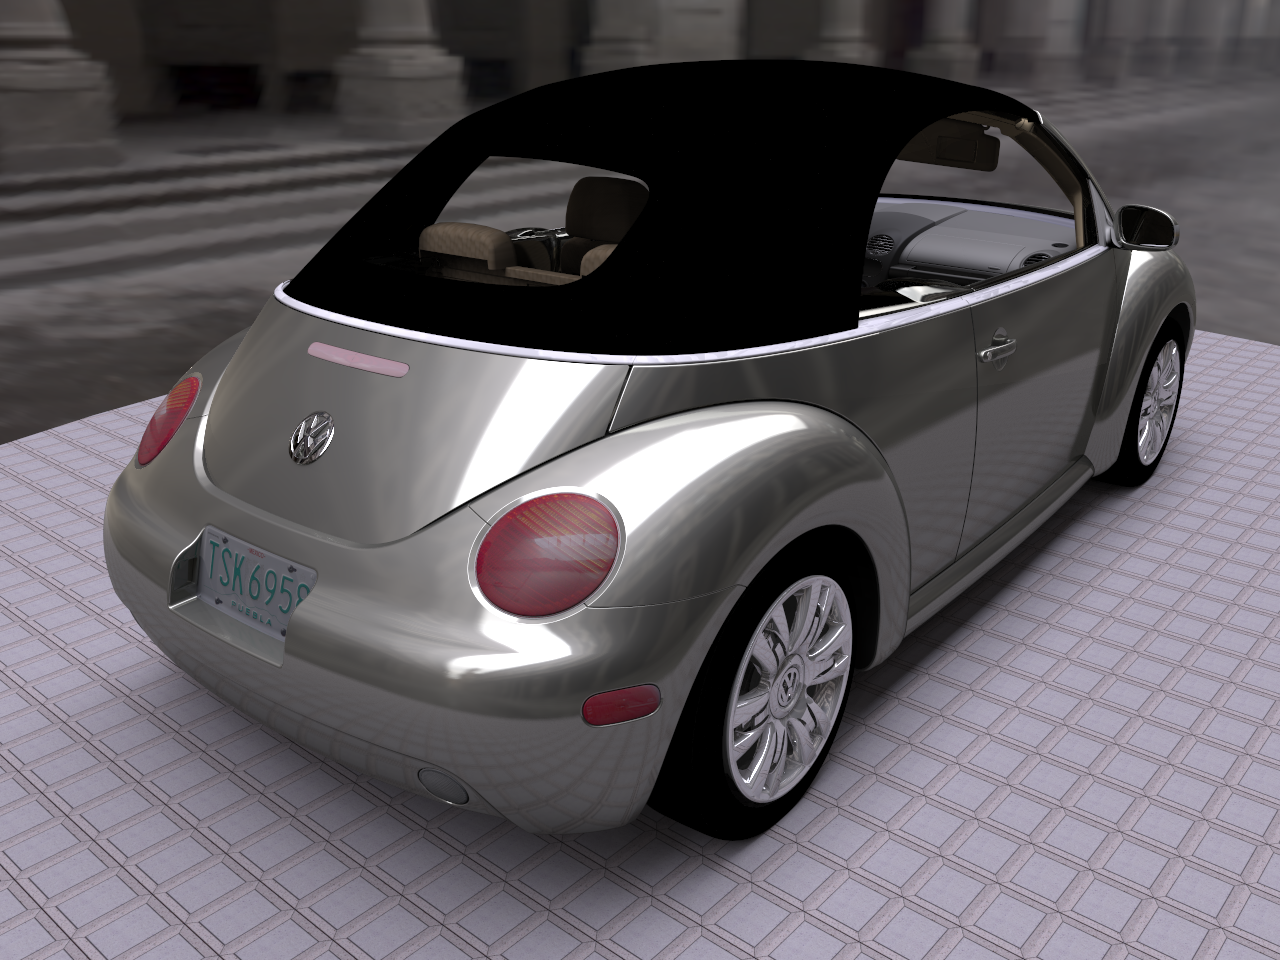
\includegraphics[width=70mm]{./img/back_hq.png}
  \end{center}
  \caption{一つめの図}
  \label{fig:one}
 \end{minipage}
 \begin{minipage}{0.75\hsize}
  \begin{center}
    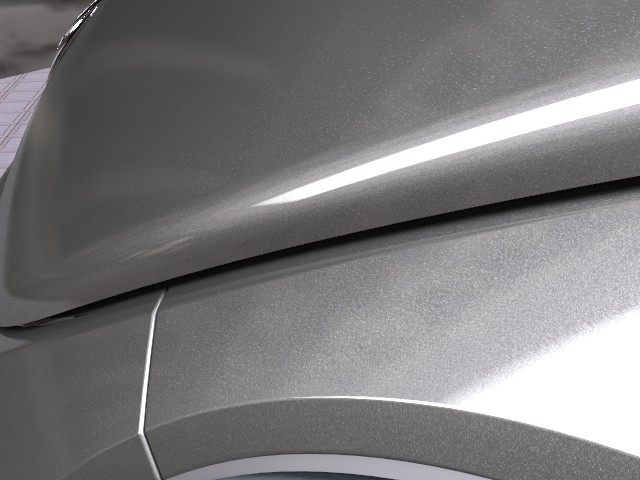
\includegraphics[width=70mm]{./img/sparkles.png}
  \end{center}
  \caption{二つめの図}
  \label{fig:two}
 \end{minipage}
\end{figure}

%% \begin{figure}[hn]
%%   \centering
%%   
\includegraphics[width=3.0in]{./img/TEMP}
%%   \caption{rumpのやつ}
%%   \label{F}
%% \end{figure}

\begin{figure}[htbp]
 \begin{minipage}{0.4\hsize}
  \begin{center}
   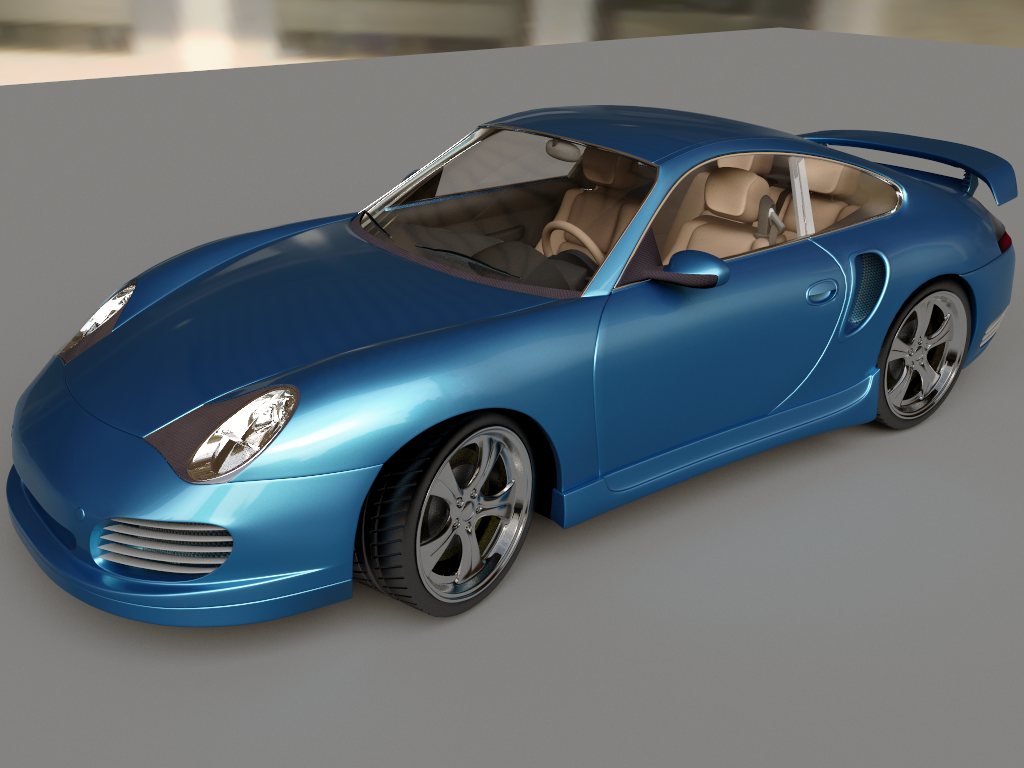
\includegraphics[width=70mm]{./img/porsche01.png}
  \end{center}
  \caption{一つめの図}
  \label{fig:one}
 \end{minipage}
 \begin{minipage}{0.75\hsize}
  \begin{center}
    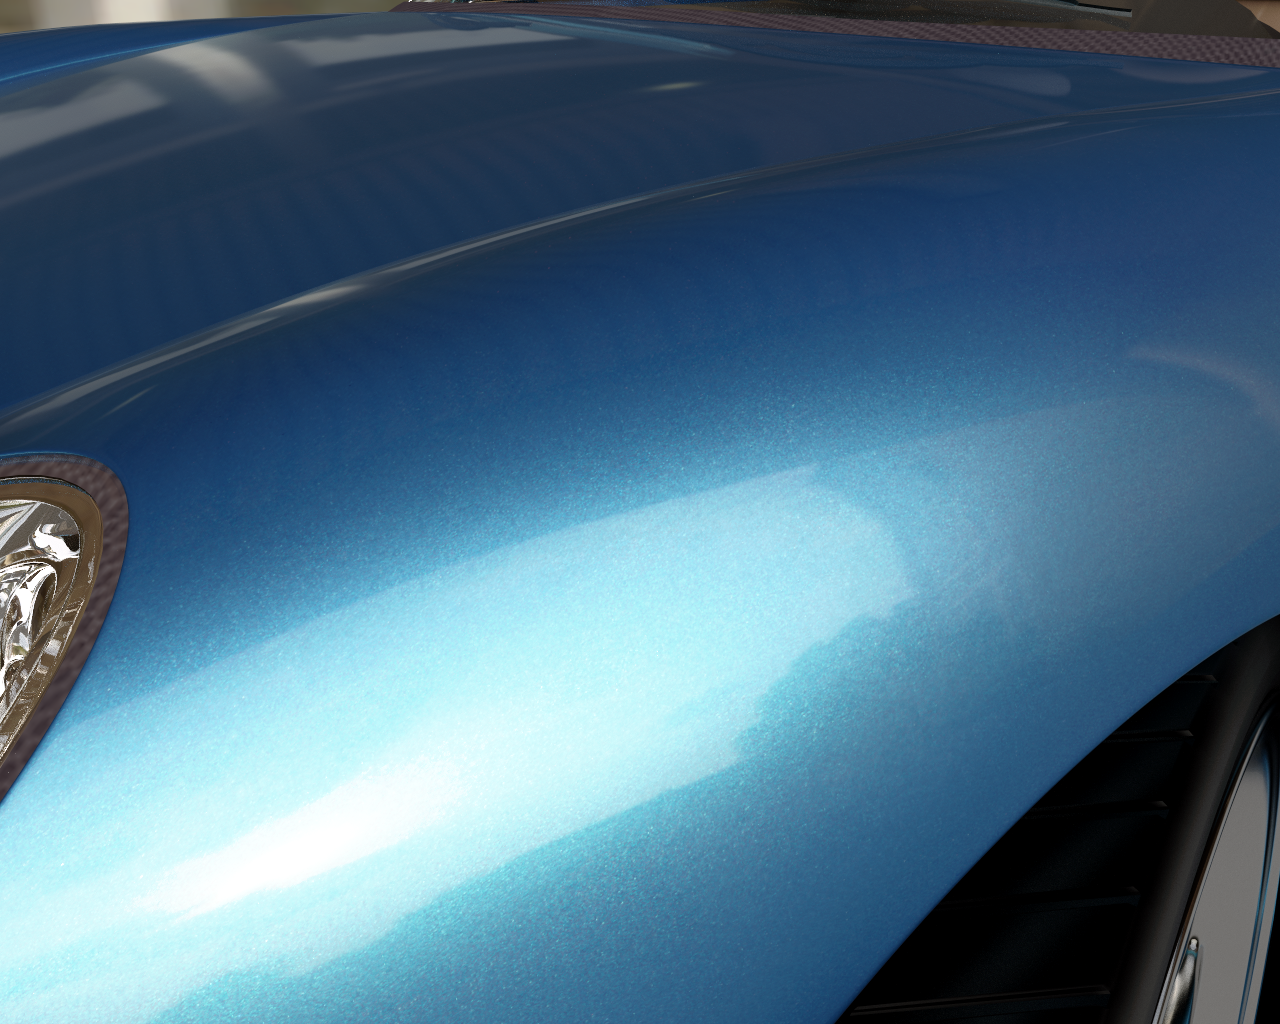
\includegraphics[width=70mm]{./img/porsche03.png}
  \end{center}
  \caption{二つめの図}
  \label{fig:two}
 \end{minipage}
\end{figure}

\noindent
また、Wenzelら\cite{}の行ったハイヒールの表面やクリスマスオーナメントのようにきらめく材質のレンダリングに関する研究では、サーフェスもしくは観測者の動きに合わせて変化するきらめきのランダムなパターンを表現している。
この手法の対象は鏡のような薄片を含むダイナミックにきらめく表面材質、およびかすかに小さいスケールのきらめきを示す粗い表面材質である。
これらの現象は原則的にはG\"{u}ntherらのように高解像度のノーマルマップによって表現することができる。
しかし、細かな特徴をもつマップは角度のついた照明条件下ではエイリアシング(aliasing)において重大な問題を抱えてしまう。
それゆえ、Wenzelらは通常では連続しているマイクロファセットの分布をサーフェス上の離散的な散乱粒子の分布と置き換えた、確率論的なモデルを提唱している。
この確率論的な階層では、個別の粒子を考えることなく多数のランダムな粒子の存在下で効率的な評価を行うことができ、それによってマルチスケールにおいて双方向反射率分布関数(BRDF: Bidirectional Reflectance Distribution Function)を導くことができる。

\begin{figure}[hn]
  \centering
  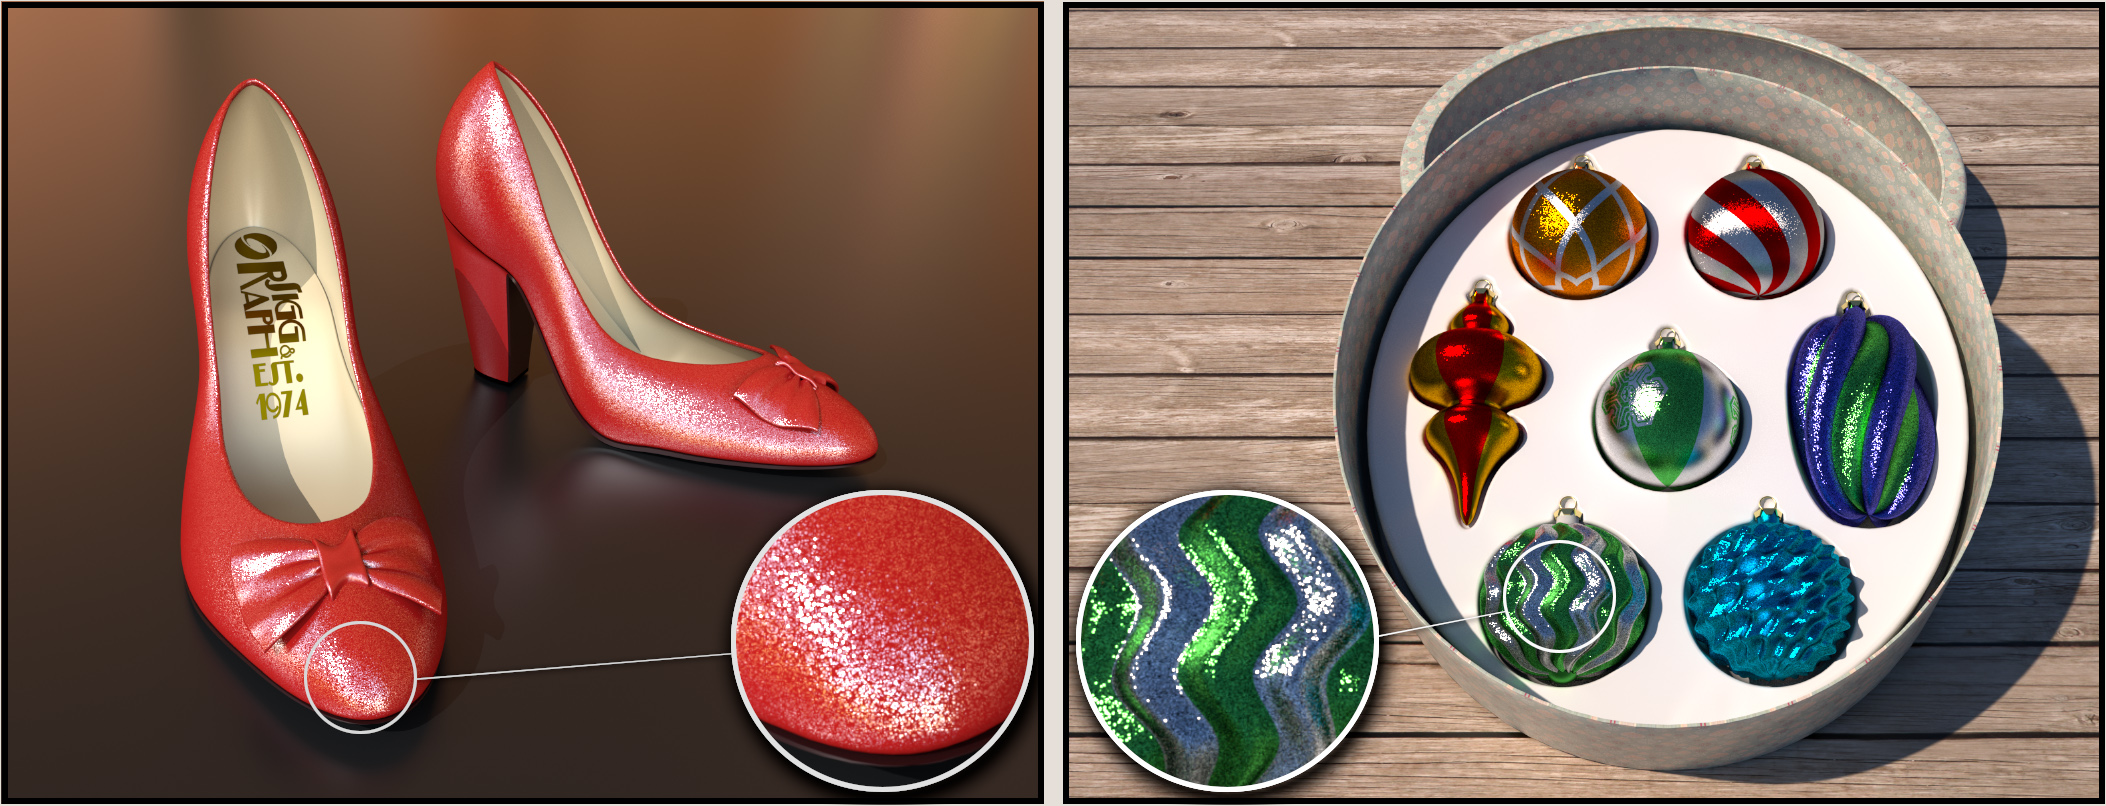
\includegraphics[width=5.0in]{./img/heel_ornament.jpg}
  \caption{ハイヒールとオーナメントの絵}
  \label{F}
\end{figure}


\subsection{構造色をいくつか}



\subsection{織り目のレンダリングに関するやつ}

織布は織糸の小さいスケールの立体構造によって変化するさまざまな外観を有する。
その構造的なディティールを正確にモデリングすることで非常にリアリスティックな織布のレンダリングをすることができるが、織糸レベルのボリューメトリック(volumetric)なモデルを作成するには非常にコストがかかる。

Zhaoら\cite{}は織糸の立体構造を自由に構築するために、詳細な生地サンプルをスキャンするのではなく、シンプルな織り構造の生地サンプルをスキャンすることによってボリューメトリックな標本のデータベースを作成し、それらからデータをコピーすることによって目的のボリュームデータを合成している。
その結果、統一的にさまざまな織りの布を表現することができ、大小のスケールの両方で非常にリアルな出力画像を生み出すことができている。

\begin{figure}[htbp]
 \begin{minipage}{0.4\hsize}
  \begin{center}
   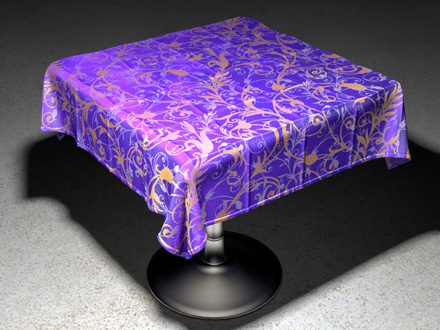
\includegraphics[width=70mm]{./img/mft_purple_cloth_ld.jpg}
  \end{center}
  \caption{一つめの図}
  \label{fig:one}
 \end{minipage}
 \begin{minipage}{0.75\hsize}
  \begin{center}
    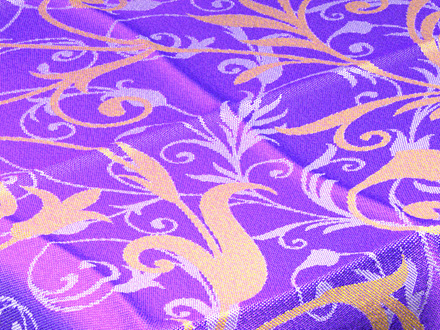
\includegraphics[width=70mm]{./img/mft_zoom_ld.jpg}
  \end{center}
  \caption{二つめの図}
  \label{fig:two}
 \end{minipage}
\end{figure}

\begin{figure}[htbp]
  \centering
  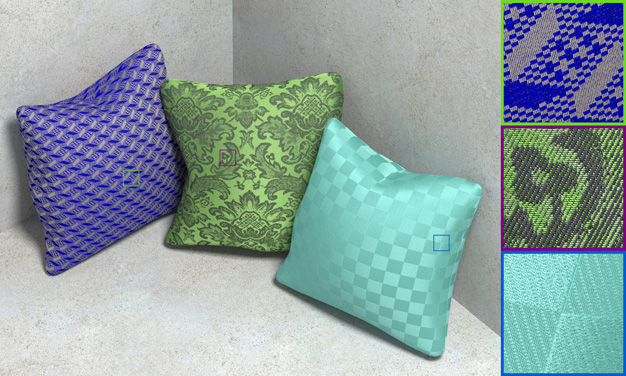
\includegraphics[width=5.5in]{./img/cussions.jpg}
  \caption{クッション}
  \label{F}
\end{figure}

\section{本研究の位置づけ}
\label{SPosition}

先述のように、表面微細構造を考慮したレンダリングに関する研究はいくつか存在する。
それらは本研究で対象としている複眼のCG表現と直接的に関連する研究ではないが、いずれも微細な構造が巨視的な外観に影響する材質に関する研究であると言える。
マイクロファセットおよび構造色は表面構造を持つといえども、全体としては均一な表面材質である。
一方、織布のレンダリングに関しては、肉眼で目視可能なレベルのスケールの構造物があり、複眼と同様に一定の条件で整列した構造をしている。


\textcolor{red}{ほかのやつはたいていランダムにやってもできるけど、本研究の対象である複眼は綺麗に並んでるやつだからそう簡単にはいかないよ}
